\begin{align}
    \vec{n} =  \myvec{-\frac{1}{\sqrt{3}} \\ 1},
    \vec{A} = \myvec{0 \\ 2}.
\end{align}
Hence, 
the equation of the line is given by
\begin{align}
\myvec{-\frac{1}{\sqrt{3}}&1}\brak{ \vec{x} - \myvec{0 \\ 2}} &= 0  \\
    \text{or, }	\myvec{-\frac{1}{\sqrt{3}}&1} \vec{x}  &= 2
\end{align}
%
\iffalse
See
    \figref{fig:chapters/11/10/2/6/line}.
\begin{figure}[H]
    \centering
    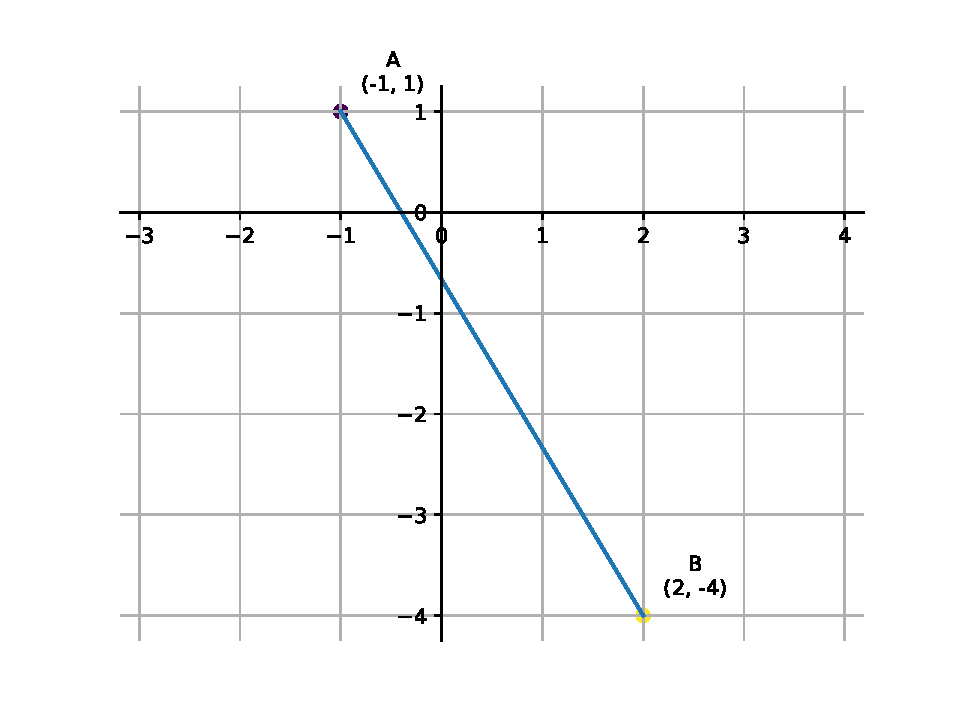
\includegraphics[width=0.75\columnwidth]{chapters/11/10/2/6/figs/fig.pdf}
    \caption{}
    \label{fig:chapters/11/10/2/6/line}
\end{figure}
\fi

